%
% File acl2018.tex
%
%% Based on the style files for ACL-2017, with some changes, which were, in turn,
%% Based on the style files for ACL-2015, with some improvements
%%  taken from the NAACL-2016 style
%% Based on the style files for ACL-2014, which were, in turn,
%% based on ACL-2013, ACL-2012, ACL-2011, ACL-2010, ACL-IJCNLP-2009,
%% EACL-2009, IJCNLP-2008...
%% Based on the style files for EACL 2006 by 
%%e.agirre@ehu.es or Sergi.Balari@uab.es
%% and that of ACL 08 by Joakim Nivre and Noah Smith

\documentclass[11pt,a4paper]{article}
\usepackage[hyperref]{acl2019}
\usepackage{times}
\usepackage{latexsym}
\usepackage{url}
\usepackage{graphicx}
\usepackage{booktabs}
\usepackage{bm}
\usepackage{amsfonts}
\usepackage{amsmath}
\usepackage{multirow}
\DeclareMathOperator*{\argmax}{arg\,max}
\DeclareMathOperator*{\argmin}{arg\,min}

\aclfinalcopy % Uncomment this line for the final submission
%\def\aclpaperid{***} %  Enter the acl Paper ID here

%\setlength\titlebox{5cm}
% You can expand the titlebox if you need extra space
% to show all the authors. Please do not make the titlebox
% smaller than 5cm (the original size); we will check this
% in the camera-ready version and ask you to change it back.

\newcommand\BibTeX{B{\sc ib}\TeX}

\newcommand{\dpcomment}[1]{\textcolor{green}{[#1 --deric]}}
\newcommand{\jbcomment}[1]{\textcolor{orange}{[#1 --josh]}}

\title{Syntactically Informed Natural Language Inference}

\author{
  Deric Pang \quad
  Joshua Bean \\
  Paul G. Allen School of Computer Science \& Engineering \\
  University of Washington \\
  Seattle, WA, USA \\
  {\tt \{dericp, jbean96\}@cs.washington.edu} \\
}

\date{}

\begin{document}
\maketitle
\begin{abstract}
We demonstrate the importance of syntactic information in semantic models by extending the
decomposable attention model for natural language inference.
By pipelining the hidden states of a neural syntax parser into the decomposable
attention model, we achieve greater performance on the SciTail dataset
than the ESIM model and DA + ELMo.
\end{abstract}

\section{Introduction}

Natural language inference (NLI) is the task of characterizing entailment and
contradiction relationships between texts.
In general, most NLI tasks are formulated as characterizing the relationship
between a pair of sequences---a premise and a hypothesis. An NLI model should
predict whether the hypothesis is entailed by the premise, contradicts the
premise, or is neutral to the premise.

We extend the decomposable attention (DA) model from  \citet{Parikh2016-em} by
incorporating syntactic features.
The DA model obtained state-of-the-art results on the
SNLI \citep{Bowman2015-is} dataset at its time of publication while using
drastically fewer parameters than previous NLI models.
We primarily
evaluate on the domain-specific SciTail dataset \citep{Khot2018-th}
for both its smaller size and lack of annotation artifacts when compared to SNLI
\citep{Gururangan2018-lj}.

Our model, \texttt{syntail}, achieves 4.8\% better 
test accuracy than the vanilla
DA model and 1.9\% better test accuracy than DA with ELMo \citep{Peters2018-fz}
all while maintaining the core DA architecture.

\section{Decomposable Attention Model}

The DA model is a simple and easily parallelizable approach to NLI.
We summarize it here so we can build upon it later.
The model
decomposes into attend, compare, and aggregate steps.

Let
$\bm{p} = \langle p_1, \dots, p_{\ell_p} \rangle$ and
$\bm{h} = \langle h_1, \dots, h_{\ell_h} \rangle$ where each $p_i, h_j \in \mathbb{R}^d$
is a $d$-dimensional word embedding vector.

\paragraph{Attend.} Compute unnormalized attention weights $e_{ij}$ with
a feed-forward neural network $F$:
\begin{align}\label{eq:attend}
    e_{ij} := F(p_i)^\mathsf{T} F(h_j).
\end{align}
Compute the aligned subphrases $\bm{H}i$ and $\bm{P}_j$:
\begin{align}
    \bm{H}_i &:= \sum_{j=1}^{\ell_h}\frac{\exp{(e_{ij})}}
                                        {\sum_{k=1}^{\ell_h}\exp{(e_{ik})}}h_j\,, \notag \\
    \bm{P}_j &:= \sum_{i=1}^{\ell_p}\frac{\exp{(e_{ij})}}
                                        {\sum_{k=1}^{\ell_h}\exp{(e_{ik})}}p_i\
\end{align}
where $\bm{H}_i$ is the weighted sum over $\bm{h}$ that aligns to $p_i$ and vice versa
for $\bm{P}_j$.

\paragraph{Compare.} Compare each $(p_i, \bm{H}_i)$ and $(h_j, \bm{P_}j)$ pairs
with another feed-forward neural network $G$:
\begin{align}
    \bm{v}^p_i &:= G([p_i, \bm{H}_i])\quad \forall i \in [1,\ldots, \ell_p]\,, \notag \\
    \bm{v}^h_j &:= G([h_j, \bm{P}_j])\quad \forall j \in [1,\ldots, \ell_h]\,.
\end{align}

\paragraph{Aggregate.} Aggregate each set of comparison vectors:
\begin{align}
\bm{v}^p = \sum_{i=1}^{\ell_p} \bm{v}^p_i \qquad\,, \qquad
\bm{v}^h = \sum_{j=1}^{\ell_h}  \bm{v}^h_j\,.
\end{align}
and make a prediction with a final feed-forward layer $H$:
\begin{align}\label{eq:predict}
    \hat{\bm{y}} = H([\bm{v}^p, \bm{v}^h]).
\end{align}

\section{Our Model}

The motivation for incorporating syntactic information in an NLI model
can be demonstrated with a simple example. Consider the premise ``Adrian is running
and Alex is swimming." If we present the DA model trained on SNLI with the
hypothesis ``Adrian is swimming," it will confidently predict that this
blatantly incorrect hypothesis is entailed by the premise. Observing
any syntactic parse of
the premise will make it obvious that Adrian is in fact running.

We experiment with features produced by two syntax parsers---the
minimal span-based neural constituency parser \citep{Stern2017-co} and
the deep biaffine attention model for dependency parsing \citep{Dozat2016-gs}. We also experiment
with different methods of incorporating the syntactic features extracted
from these parsers.

\subsection{Extracting Syntactic Information}

The minimal span-based neural constituency parser and the deep biaffine attention
model for dependency parsing both encode the input sequence with an LSTM. Using
this LSTM, we obtain
syntactic features $\bm{s}^p = \langle s^p_1, \dots, s^p_{\ell_p} \rangle$ and
$\bm{s}^h = \langle s^h_1, \dots, s^h_{\ell_h} \rangle$ from the premise and hypothesis,
respectively. An $s_i$ is either
the final hidden state $\bm{r}_i$ of the LSTM at index $i$ or a projected
representation of $\bm{r}_i$.

\subsection{Syntail Architectures}

We will now describe the different model architectures we experimented with.
In general, as the version number increases, the complexity of the model increases.

\paragraph{v1: Naive late fusion of syntactic features.}
The simplest way to incorporate $\bm{s}$ is to concatenate its final representation to
$\bm{v}^p$ and $\bm{v}^h$ as shown in figure~\ref{fig:v1}.

\begin{figure}[h]
    \centering
    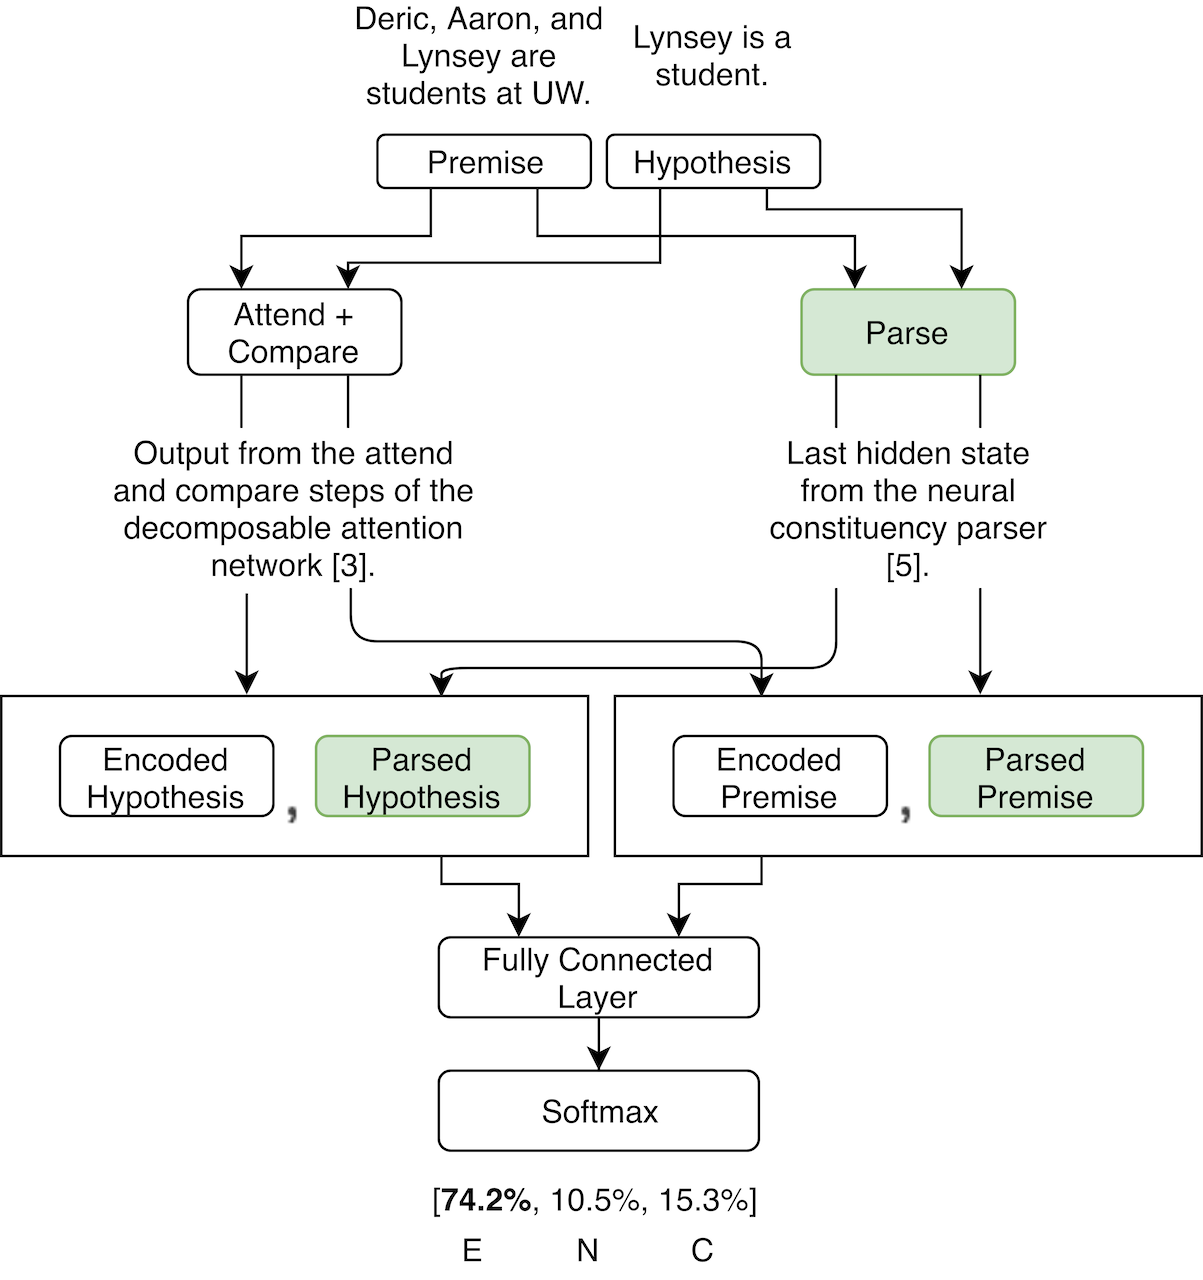
\includegraphics[width=\linewidth]{figures/v1.png}
    \caption{Syntail v1 architecture.}
\label{fig:v1}
\end{figure}

The prediction step in equation~\ref{eq:predict} then becomes:
\begin{align}
    \hat{\bm{y}} = H([\bm{v}^p, s^p_{\ell_p}, \bm{v}^h, s^h_{\ell_h}])
\end{align}
where we concatenate the final hidden representation of the premise and hypothesis
when passed through the neural syntax parser with the aggregrated comparision vectors.
Everything else is identical to the DA model.

\paragraph{v2: Using syntactic features to attend.}
We wanted to experiment with incorporating syntactic features earlier in the model.
Instead of learning weights on the syntactic features, it is possible to
concatenate them to the projected input representations as show in figure~\ref{fig:v2}.

\begin{figure}[h]
    \centering
    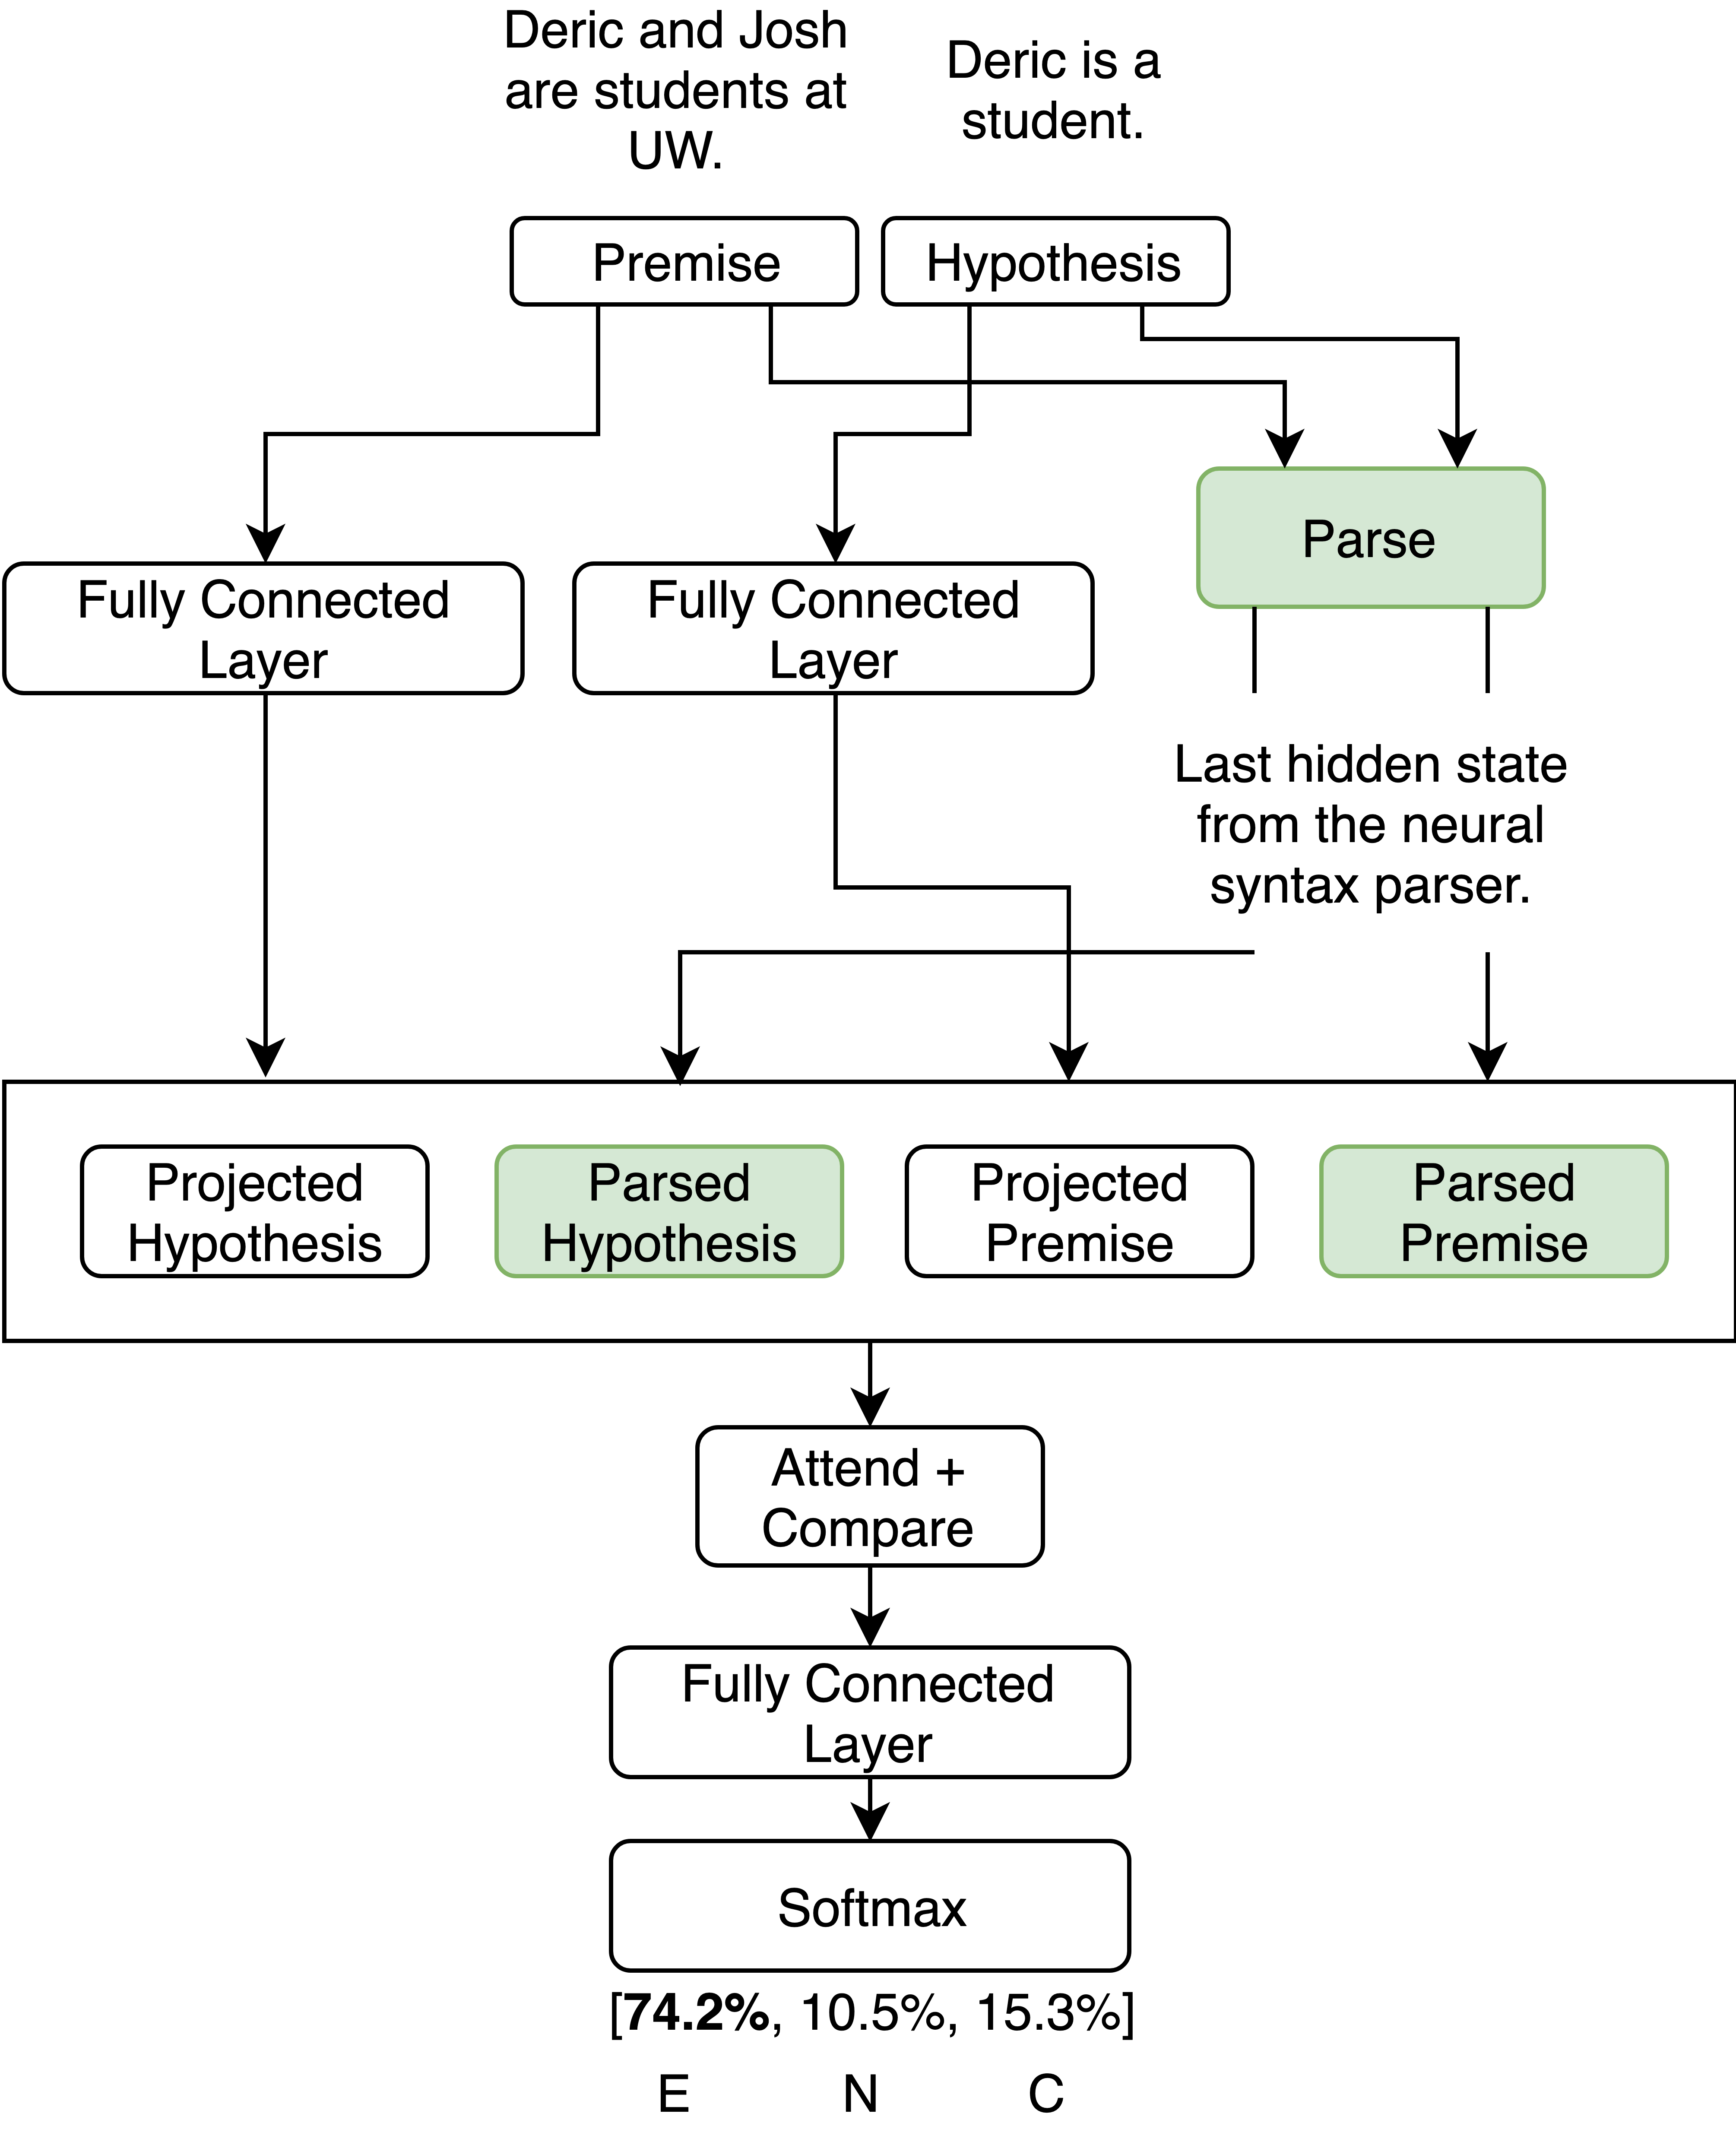
\includegraphics[width=\linewidth]{figures/v2.png}
    \caption{Syntail v2 architecture.}
\label{fig:v2}
\end{figure}

Computing the
unnormalized attention weights in equation~\ref{eq:attend} then becomes:
\begin{align}
    e_{ij} := [F(p_i), s^p_i]^\mathsf{T} [F(h_j), s^h_i]
\end{align}
where instead of calculating the alignment using only the 
projected hypothesis and premise vectors, we now also use the final hidden states of
the premise and hypothesis when passed through the neural syntax parser.
This seems rather naive since this model will not
learn any weights on the syntactic features, but in practice this model
performs very well. Everything else is identical to the DA model.

\paragraph{v3: Using syntactic features to project the premise and hypothesis.}
We decided to try incorporating the syntactic features even earlier in the model.
Instead of concatenating the final hidden states of the parsed premise and hypothesis
with the projected inputs, we concatenate the final hidden states of the parsed
premise and hypothesis with the inputs immediately before projecting them. This
architecture is shown in figure~\ref{fig:v3}.

\begin{figure}[h]
    \centering
    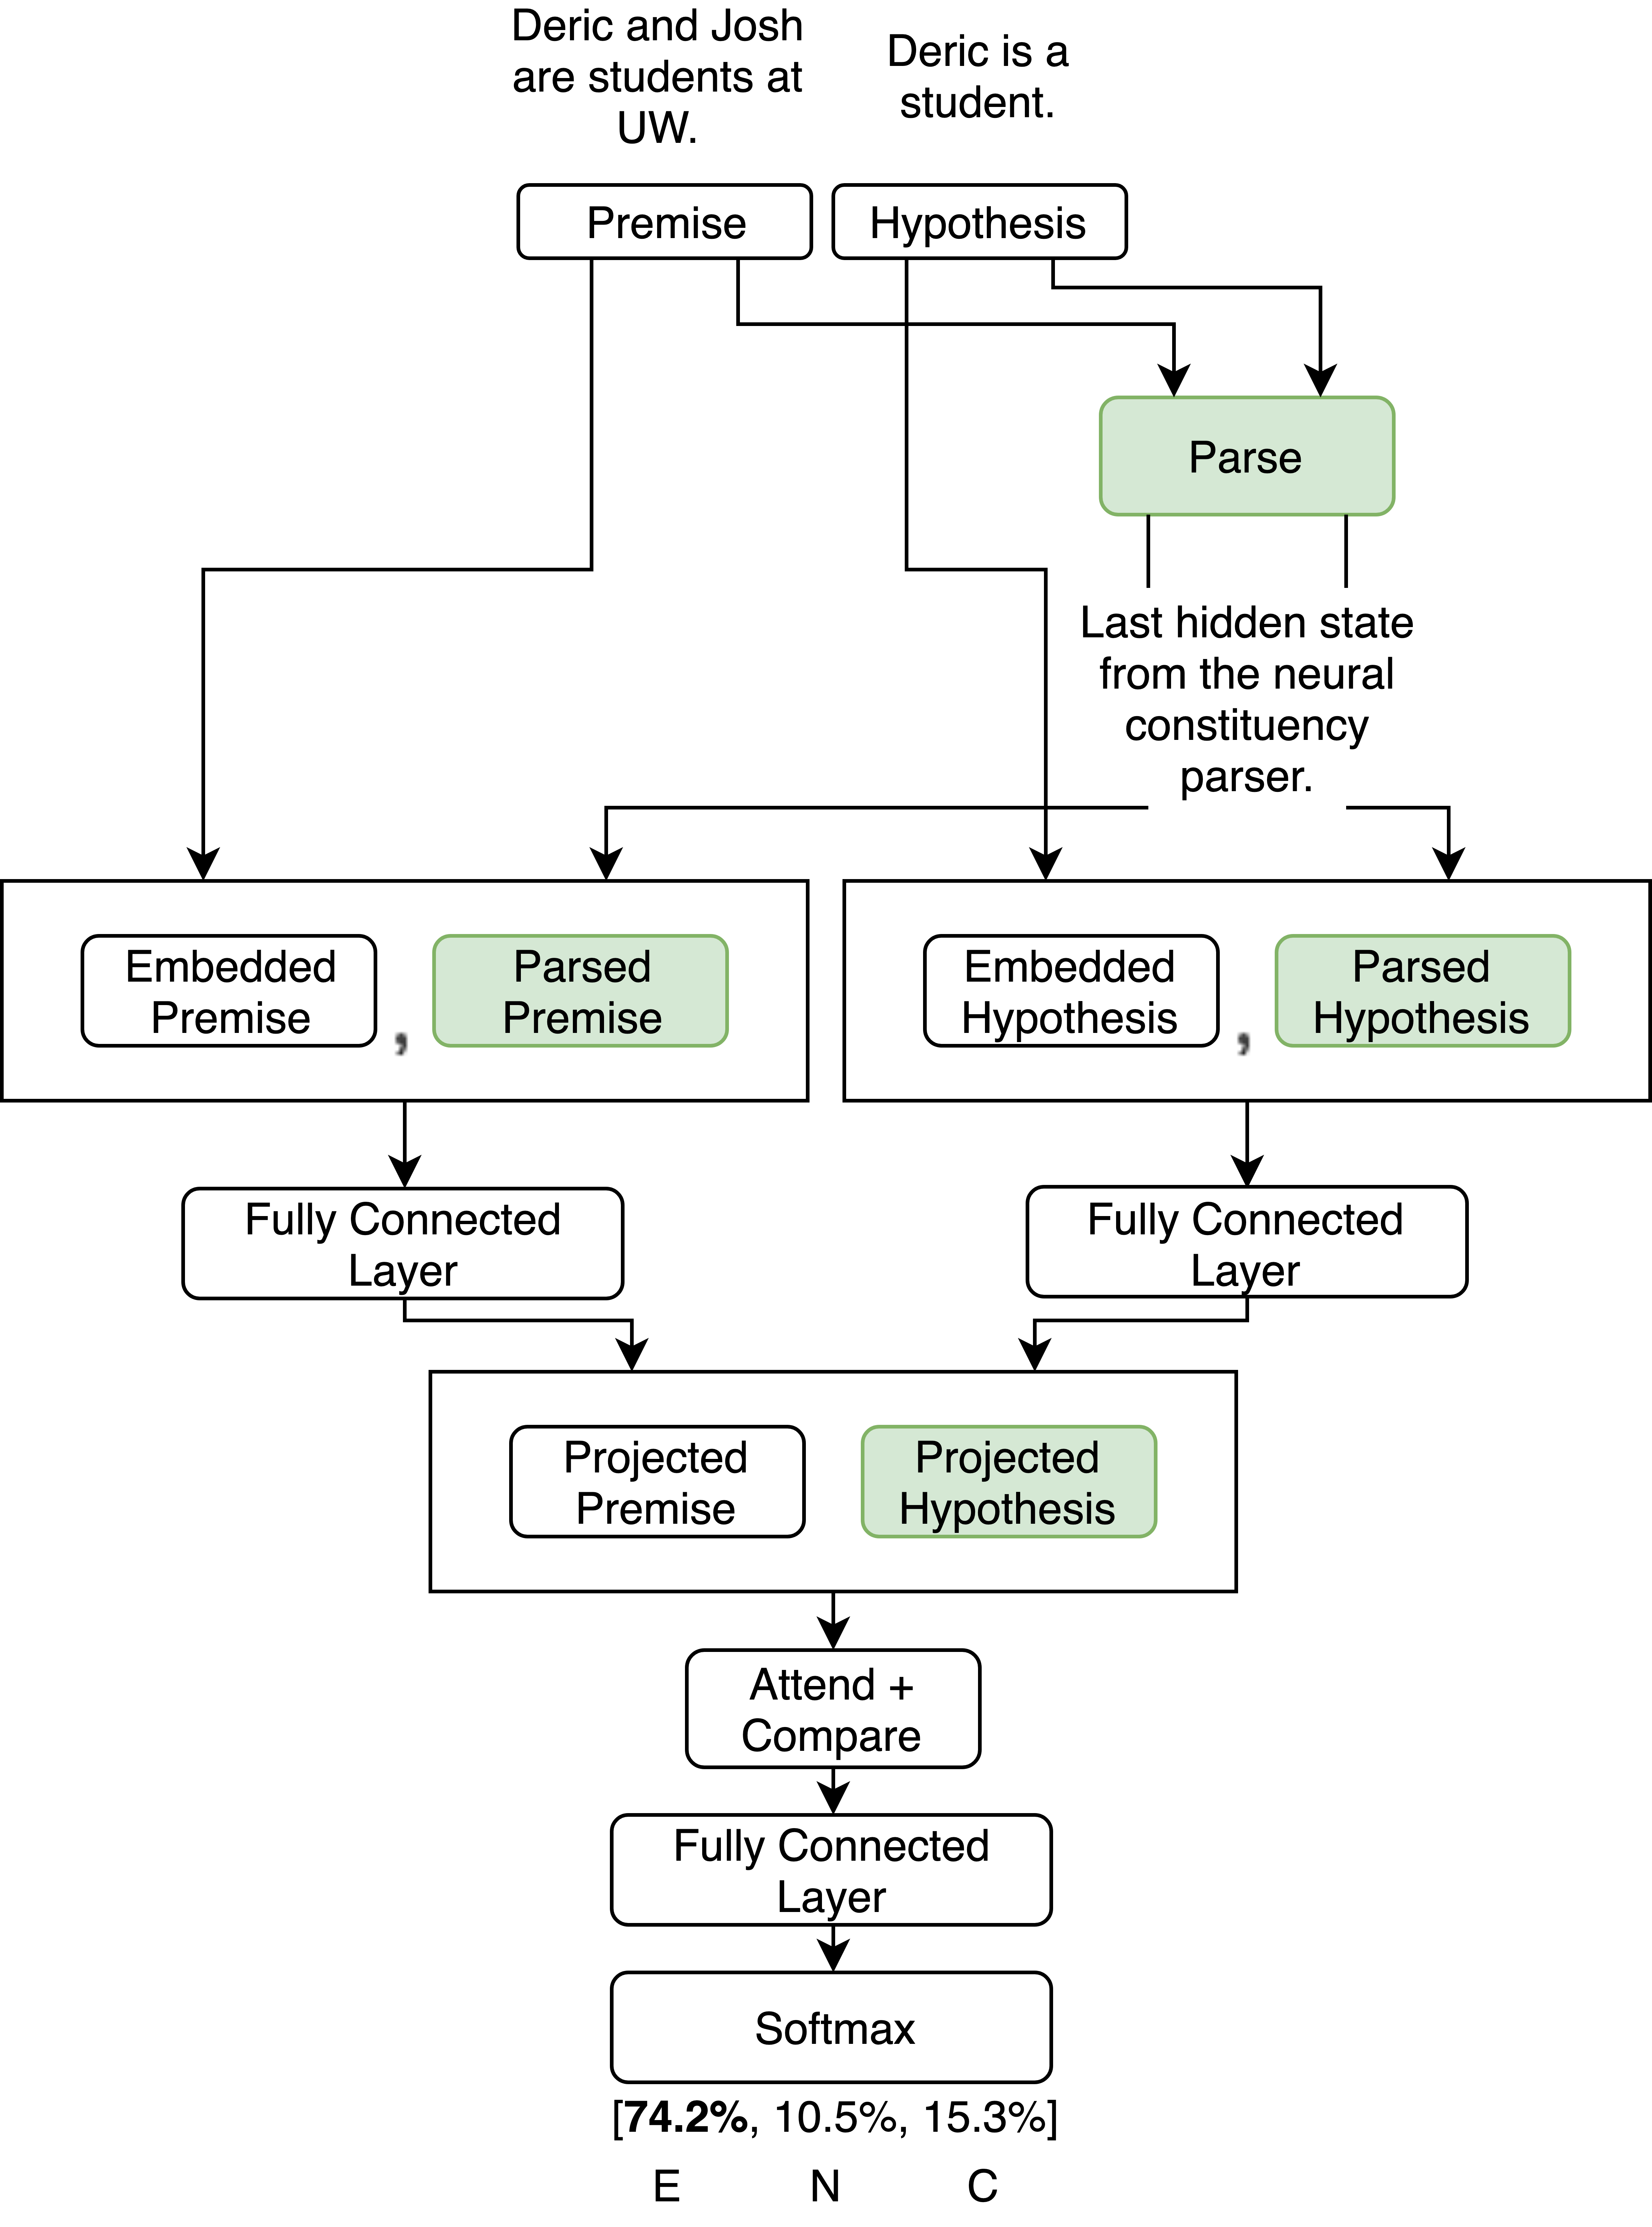
\includegraphics[width=\linewidth]{figures/v3.png}
    \caption{Syntail v3 architecture.}
\label{fig:v3}
\end{figure}

Computing the unnormalized attention weights in equation~\ref{eq:attend} then becomes:
\begin{align}
    e_{ij} := F([p_i, s^p_i])^\mathsf{T} F([h_j, s^h_j]).
\end{align}
Everything else is identical to the DA model.

\paragraph{v4: Projecting the syntactic features before computing attention.}
After noticing a drop in performance from v2 to v3, we hypothesized that it was
due to not allowing our model to transform the syntactic features enough before
calculating attention.
We decided to learn weights to project the final hidden states of the parsed
premise and hypothesis by passing them through an additional fully-connected layer before 
concatenating them to the inputs. This architecture is shown in figure~\ref{fig:v4}

\begin{figure}[h]
    \centering
    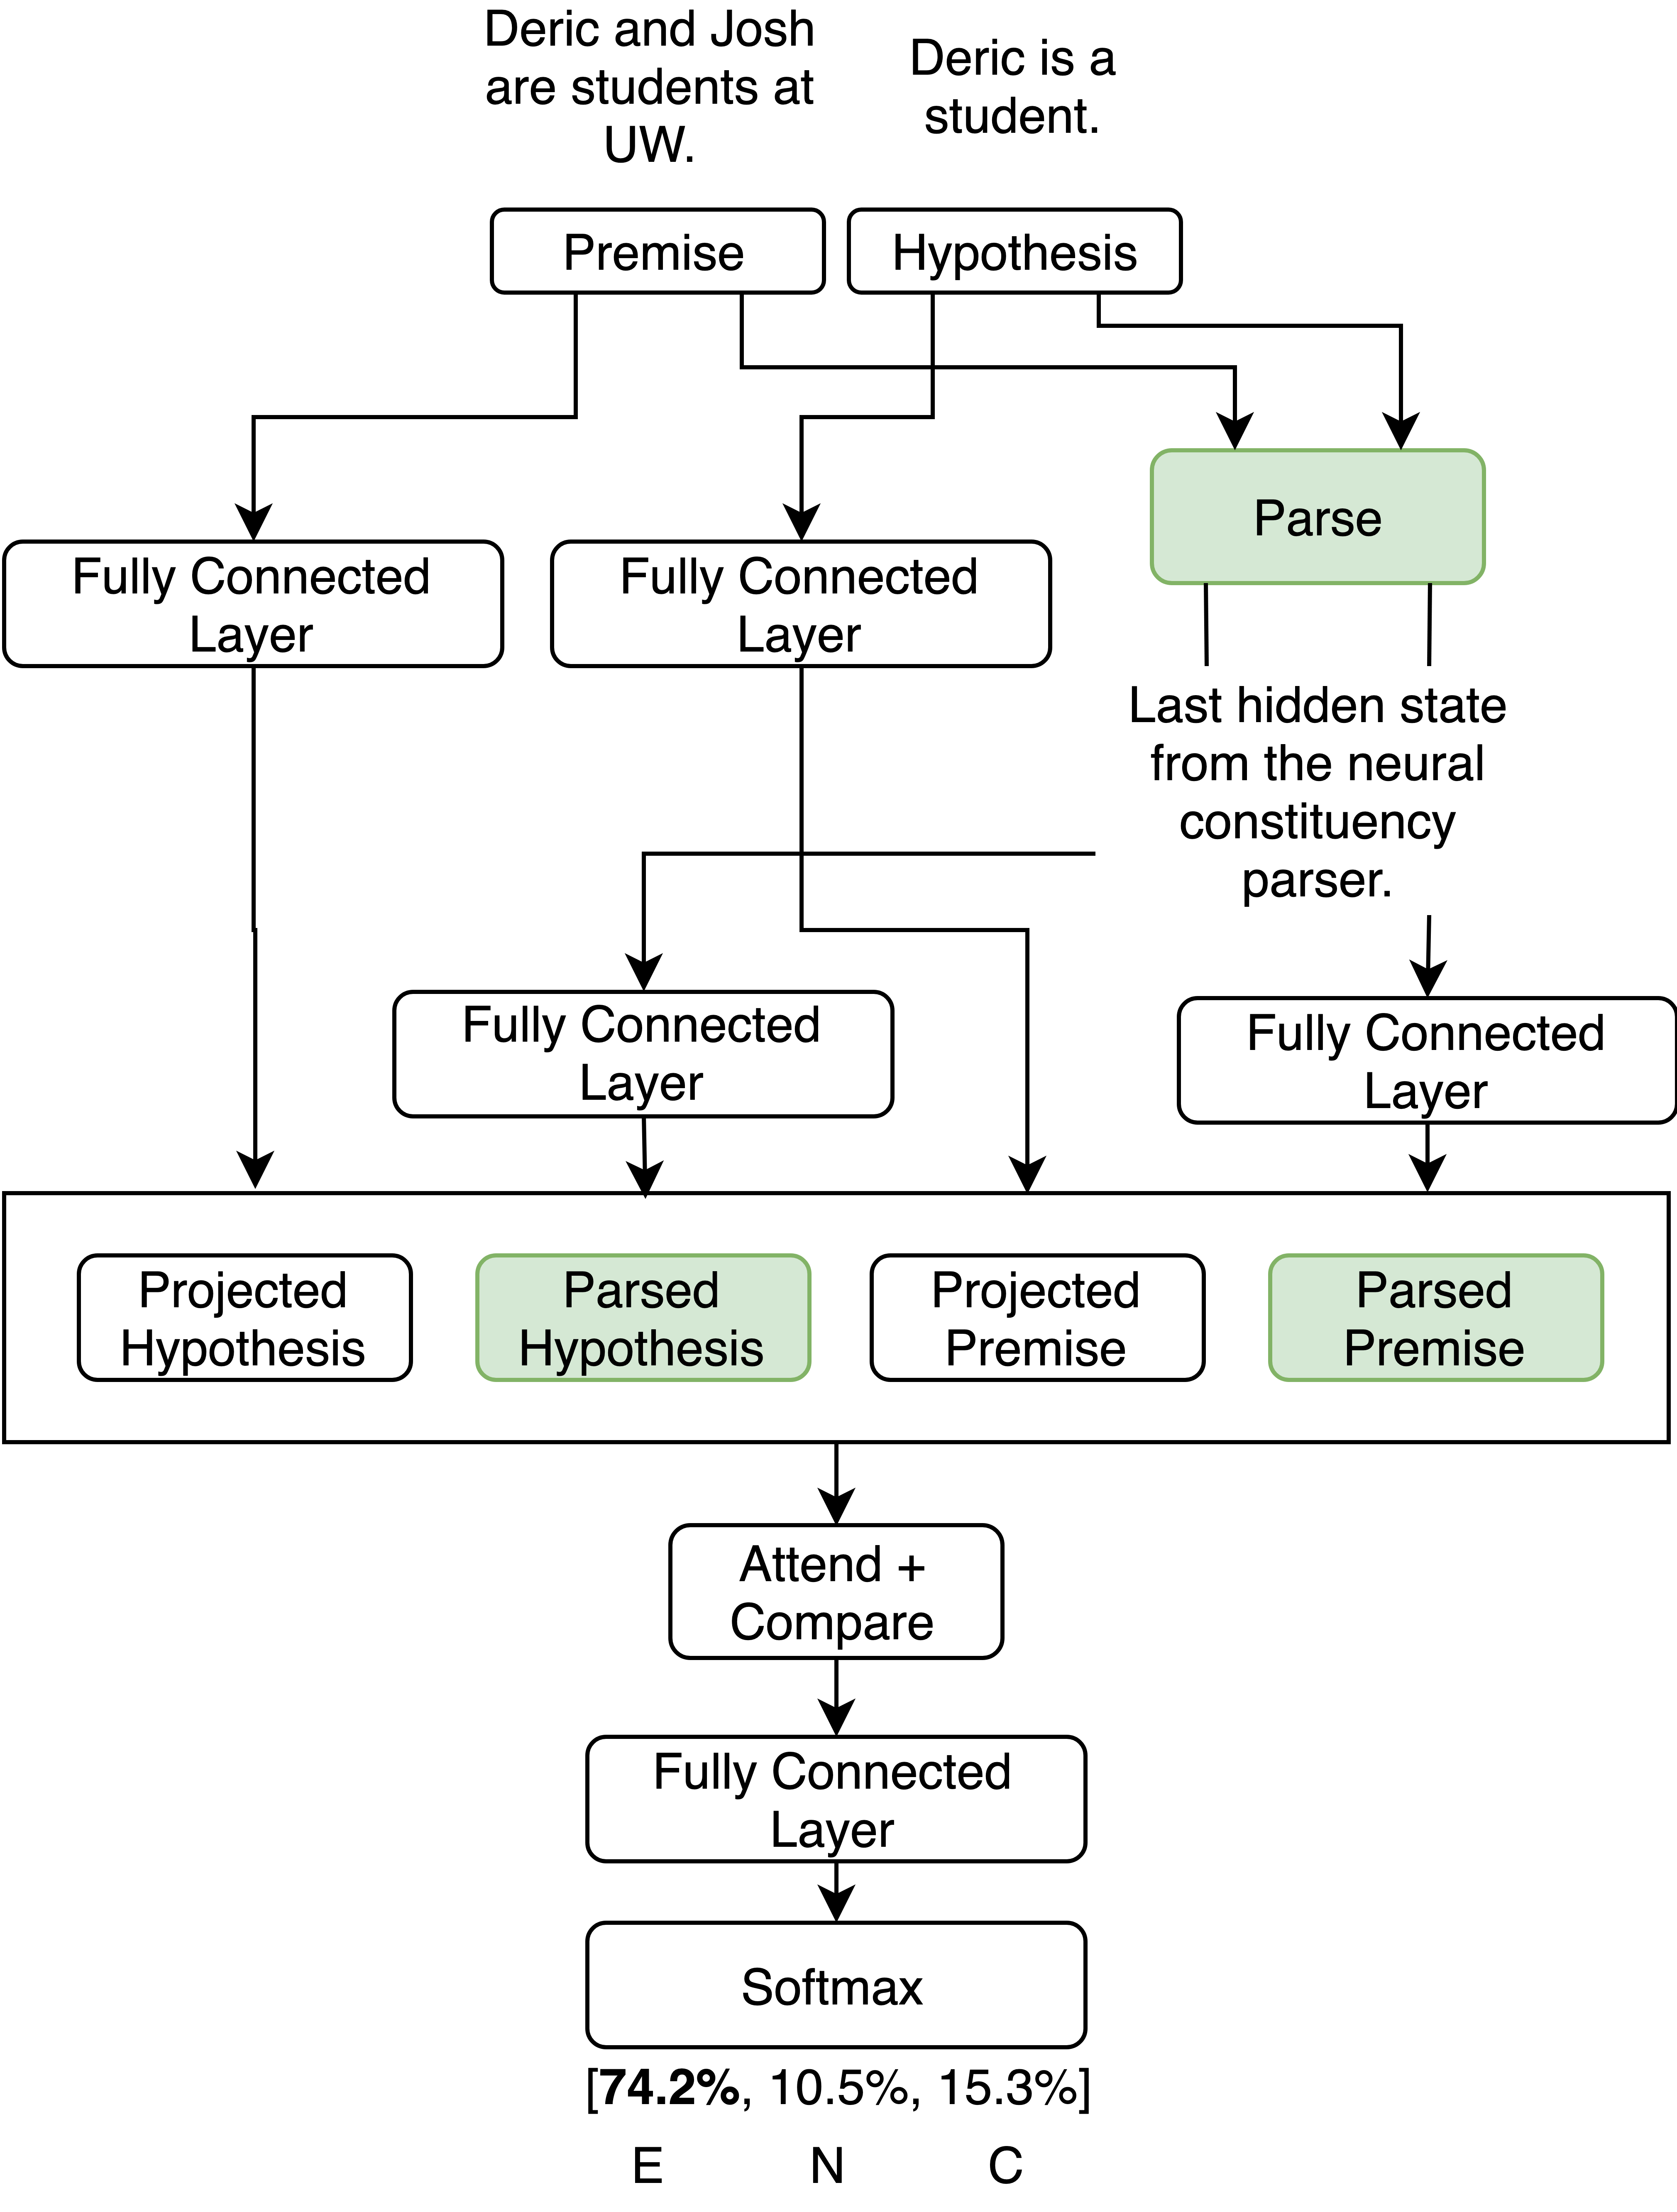
\includegraphics[width=\linewidth]{figures/v4.png}
    \caption{Syntail v4 architecture.}
\label{fig:v4}
\end{figure}

Computing the unnormalized attention weights in equation~\ref{eq:attend} then becomes:
\begin{align}
    e_{ij} := F([p_i, J(s^p_i)])^\mathsf{T} F([h_j, J(s^h_j)])
\end{align}
where $J$ is a feed-forward neural network.
Everything else is identical to the DA model.

% \jbcomment{If we're only using data from the dependency parser we should probably 
% remove the section following this comment}
% Supplemental variations were done on top of these restructures of the network. One 
% of the variations that we introduced was a retrained constituency parser. By 
% retraining the constituency parser on the Penn Treebank dataset \citep{marcus1993building} 
% we could change the dimensions of the encoded syntax vectors to better fit with our models. 
% Additionally, we experimented with training our models using the dependency parser model 
% derived by \citet{Dozat2016-gs} to see if the different types of encoded parses influenced 
% the performance of the network.

\subsection{Implementation Details}

\subsubsection{Word Embeddings}

Due to resource constraints, we limited our models to only use 300-dimensional
6B GloVe word embeddings \citep{Pennington2014-uo}.
Additionally, contextual embeddings are known to capture syntax in some capacity,
so limiting our models to only use GloVe vectors
made it easier to experiment with the syntactic features in isolation.

\subsubsection{Neural Syntax Parser}

We initially used a constituency parser in syntail. However,
after some experimentation, we found that we were achieving better results
with a dependency parser.
For this reason, we only report results using the deep biaffine attention
model for dependency parsing.
Dependency parsers focus on encoding the
the relationships between words as opposed to determining constituents.
Intuitively, if we consider our example sentence, ``Adrian is running and Alex is swimming,''
the dependency arcs will be more informative of who is doing what.

\subsection{Hyper-parameters}

We use 200-dimensional projections of the word embeddings. Our feed-forward neural
networks are 2 layered and have hidden dimensions of 200. We train with both
Adam \citep{kingma2014adam} and Adagrad \citep{duchi2011adaptive} and report the
better result.

\section{Experiments}

We compare our model's performance to the decomposable attention model
\citep{Parikh2016-em} and the ESIM model \citep{Chen2016-wl}.
Early on in our experiments, we noticed that features from a dependency
parser seemed to perform better than those from a constituency parser.
Therefore, all of our models use the deep biaffine attention model for
dependency parsing \citep{Dozat2016-gs}.

\paragraph{Datasets.}
For practical reasons, we only experiment on the SciTail dataset. SciTail (27k pairs) is
significantly smaller than SNLI (570k pairs) \citep{Bowman2015-is} or MultiNLI (433k pairs)
\citep{Williams2017-uh} which makes it feasible to try many different
architectures given limited resources.

Additionally, \citet{Gururangan2018-lj} showed that SNLI and MultiNLI
have significant annotation artifacts whereas SciTail is the first entailment set to be
completely derived from sentences that exist ``in the wild.''

\paragraph{Baselines.}
We list baseline performance reported by \citet{Khot2018-th} of a majority class predictor,
n-gram model, and ESIM \citep{Chen2016-wl} in table~\ref{table:experiments}. We reimplemented
and retrained the DA model and obtained similar test accuracies as reported by \citet{Chen2016-wl}.
Adding ELMo to the DA model improved test accuracy performance by approximately 3\%.

\subsection{Results}

\begin{table}[h]
\centering
\resizebox{\linewidth}{!}{
\begin{tabular}{cccccc} 
\toprule
Model          & Embeddings      & Dev. Acc. & Test Acc.  \\ 
\midrule
Majority Class & n/a             & 63.3      & 60.3       \\
N-Gram         & n/a             & 65.0      & 70.6       \\
ESIM           & GloVe 840B 300d & 70.5      & 70.6       \\
DA             & GloVe 6B 300d   & 70.4      & 72.6       \\
DA             & ELMo            & 79.1      & 75.5       \\
\midrule
Syntail v1     & GloVe 6B 300d   & 78.4      & \textbf{77.4}       \\
Syntail v2     & GloVe 6B 300d   & \textbf{82.3}      & \textbf{77.4}       \\
Syntail v3     & GloVe 6B 300d   & 79.0         & 76.1          \\
Syntail v4     & GloVe 6B 300d   & 81.3      & 77.0       \\
\bottomrule
\end{tabular}}
\caption{Dev and test accuracies on SciTail.}
\label{table:experiments}
\end{table}

Our experimental results can be found in table~\ref{table:experiments}.
All of our syntail models
achieve better test accuracy than the baseline models. This demonstrates
that the syntax parser is providing features that are both useful for
determining entailment relationships and difficult for the baseline
models to learn on their own.

We were surprised that the simpler v1 and v2 models outperformed the
more complicated v3 and v4 models. This is likely due to the syntactic
information being fused later in v1 and v2. The later the features are
fused, the closer they are to the loss function and the more the model
can learn to use them.

It is also interesting that adding and additional transformation
on the syntactic features in v4 decreases performance.
Again, this is likely due to the early fusion problem.
The additional power of the model is overwhelmed by the detrimental
effects of the vanishing gradient problem.
It is also possible that the randomly initialized weights 
of the feed-forward neural network struggle to learn how to
summarize the syntactic features.

One downside of using a pretrained syntax parser is that the data SciTail is
created from (science exam questions) is in a very different domain than
the data used to create the Penn Treebank (news articles)
\citep{marcus1993building}.
This likely significantly reduces the accuracy of the syntax parser on
SciTail. Retraining the syntax parser on in-domain data
should produce better syntactic features
and further improve 
the performance of our model.

\subsection{Analysis of Syntactic Features}

We discuss a specific in-domain input example shown in table~\ref{table:example}
to better understand the effects of syntactic features. The predictions on this
input made by the DA and
syntail v1 models are shown in table~\ref{table:pred-example}.

\begin{table*}[t]
    \centering
    \resizebox{\linewidth}{!}{
    \begin{tabular}{c c}
    \toprule
    Premise & Hypothesis \\
    \midrule
    The continental crust is less dense than the mantle but the oceanic crust is not.
        & The oceanic crust is more dense than the mantle. \\
    \bottomrule
    \end{tabular}}
    \caption{A pair of sentences where syntail performs particularly well. The hypothesis is
             entailed by the premise.}
\label{table:example}
\end{table*}

\begin{table}[h]
    \centering
    \begin{tabular}{c c c}
        \toprule
         Model & Entails (correct) \\
         \midrule
         DA & 29.5\% \\
         Syntail v1 & \textbf{67.9\%} \\
         \bottomrule
    \end{tabular}
    \caption{Entailment probabilities generated by the DA and syntail v1 models on the input
             from table~\ref{table:example}.}
\label{table:pred-example}
\end{table}

Syntail v1 correctly determines the relationship of this pair of sentences
while the DA model does not.
To investigate why, we visualize the attention weights in figures~\ref{fig:da-attention-weights}
and \ref{fig:sytail-attention-weights}.
We can see that the attention produced by the DA model is nonsensical and focuses solely on
``is.'' It seems that by incorporating syntactic information, syntail v1 is forced to learn
a more reliable attention function.

\begin{figure}[h]
    \centering
    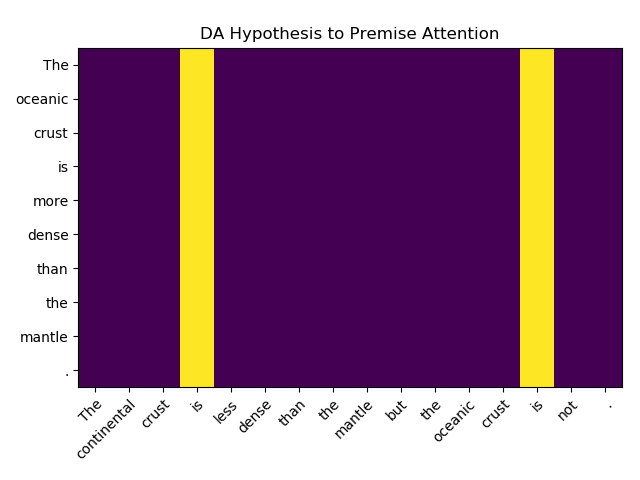
\includegraphics[width=\linewidth]{figures/da-h2p-attention.png}
    \caption{Hypothesis to premise attention weights of the DA model when processing
             the input from table~\ref{table:example}.}
    \label{fig:da-attention-weights}
\end{figure}

\begin{figure}[h]
    \centering
    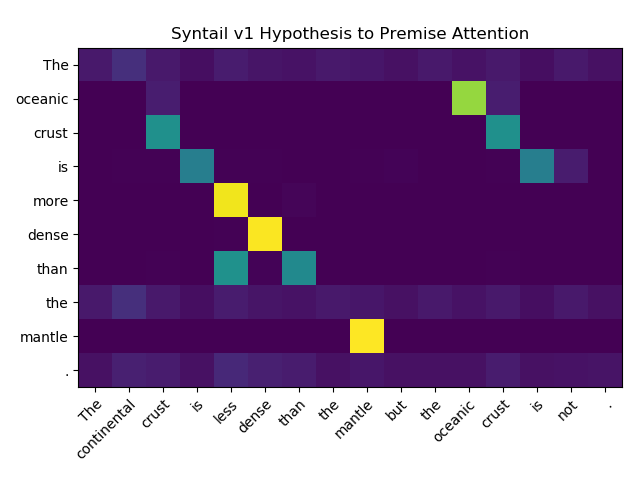
\includegraphics[width=\linewidth]{figures/syntail-h2p-attention.png}
    \caption{Hypothesis to premise attention weights of syntail v1 when processing
             the input from table~\ref{table:example}.}
    \label{fig:sytail-attention-weights}
\end{figure}

\section{Related Work}

Previous works have experimented with incorporating syntactic features for semantic tasks.
\citet{Chen2016-wl} use tree structures generated by a constituency parser to improve
their ESIM model. They encode the phrase-structure trees with a Tree-LSTM and use its
hidden states. \citet{Khot2018-th} incorporate syntactic features by
proposing a model architecture which can use any graph-based syntactic/semantic structure.

Other works have experimented with incorporating syntactic learning objectives.
\citet{Strubell2018-qw} achieved state-of-the-art performance
for a model using predicted predicates and standard word embeddings on
CoNLL-2005 SRL by performing multi-task training on additional syntactic tasks.
\citet{Swayamdipta2017-ct} use hard-coded constituency and dependency parse features
and a syntactic scaffold to
extend the softmax margin segmental RNN (segRNN) model.

\section{Conclusion}

By making simple extensions to the DA model,
our syntail models outperform ESIM and DA + ELMo model on SciTail.
Our results demonstrate the importance of syntactic information in semantic models
and motivate future research into syntactically informed models.

\bibliographystyle{acl_natbib}
\bibliography{main}

\end{document}
